\chapter{Methods}
\label{chap-methods}

\section{Disturbance models}

\subsection{Randomly-occurring deterministic disturbances}

\textit{Randomly-occurring deterministic disturbances} (RODDs) [CITE] are a family of stochastic process models suitable for simulating various types of infrequently-occurring disturbances in discrete-time.  The structure of the RODD model is

\begin{equation} \label{eq:RODD}
	p(k)= \frac{B(z^{-1})}{A(z^{-1})}w_p(k)
\end{equation}

where $p(k)$ is the generated disturbance signal, $A(z^{-1})$ and $B(z^{-1})$ are arbitrary polynomial functions of the shift operator, and $w_p(k)$ is a random variable generated by a switching system.

The following switching system can be used to generate randomly-occurring disturbances.

\begin{equation} \label{eq:alpha1}
w_p(k) \sim 
\begin{cases*}
	0 & with probability $1-\epsilon$, \\
	\mathcal{N}\left(0, \sigma_{w_p}\right) & with probability $\epsilon$.
\end{cases*}
\end{equation}

Here, $w_p(k)$ is either 0 or is sampled from a normal distribution.  When the probability $\epsilon$ is low ($\epsilon<<1$), this system produces \textit{infrequent shocks}.

Alternatively, a mixture of two distributions can be used as in (\ref{eq:alpha2}).

\begin{equation} \label{eq:alpha2}
w_p(k) \sim 
	\begin{cases*}
		\mathcal{N}\left(0, \sigma_{w_p}\right) & with probability $1-\epsilon$, \\
		\mathcal{N}\left(0, b\sigma_{w_p}\right) & with probability $\epsilon$.
	\end{cases*}
\end{equation}

In this case, $\sigma_{w_p}$ is small and $b$ is typically large so that the magnitude of the random shocks is much greater than the random noise that occurs between shocks.

Figure \ref{fig:alpha-pdf} illustrates the probability density of $w_p$ in the case of (\ref{eq:alpha2}) with $\sigma_{w_p}=0.01$, $b=100$, and $\epsilon=0.01$. Although it is difficult to tell from the plot, this is a mixture distribution with two overlapping components. The component that generates the infrequent shocks is barely visible because of its low probability. While 99 percent of the probability density lies within a narrow range (-0.036 < $w_p(k)$ < 0.036), the so-called shocks, which occur with probability 0.01, have much higher amplitude ($b\sigma_{w_p}=1$).

\begin{figure}[htp] \label{fig:alpha-pdf}
	\centering
	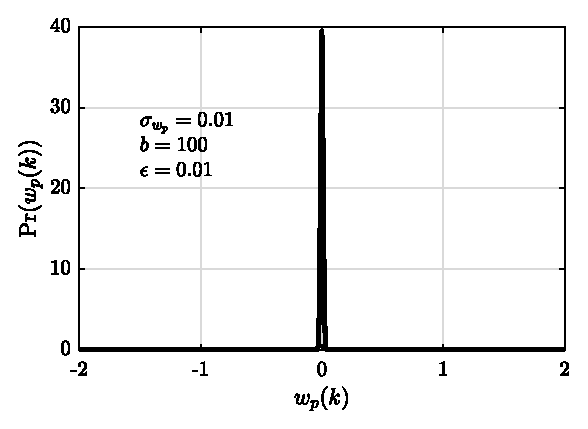
\includegraphics[width=9cm]{alpha-pdf-4.eps}
	\caption{Probability density of a random shock signal}
\end{figure}

The choice of $A(z^{-1})$ and $B(z^{-1})$ in (\ref{eq:RODD}) determines the nature of the RODD disturbance. For example, if $B(z^{-1})=1$ and $A(z^{-1})=1-z^{-1}$, $p(k)$ will be a random walk process with infrequent, large step changes, such as example (a) in Figure \ref{fig:RODDstep}.

\begin{figure}[htp] \label{fig:RODD-examples}
	%... figure contents...
\end{figure}

Denoting $\nabla=1-z^{-1}$, the \textit{RODD step-disturbance} process can be defined as

\begin{equation} \label{eq:RODD-step}
	p(k)= \frac{1}{\nabla}w_p(k)
\end{equation}

The following produces a \textit{RODD ramp-disturbance} consisting of a series of ramps with randomly-occurring changes in slope.

\begin{equation} \label{eq:RODD-ramp}
	p(k)= \frac{1}{\nabla^2}w_p(k)
\end{equation}

The following process with $0<a_1<1$ produces a RODD disturbance consisting of randomly-occurring decaying exponential changes.

\begin{equation} \label{eq:RODD-exp}
	p(k)= \frac{1}{(1-a_1z^{-1})\nabla}w_p(k)
\end{equation}

Examples of these RODD disturbances are also shown in Figure \ref{fig:RODDstep}.

\subsection{Hidden Markov Models}

The basic RODD model described above can be extended using a \textit{hidden Markov model} (HMM) to describe the switching behaviour [CITE WONG \& LEE 2009]. A Markov model is a stochastic model of a system with discrete states in which it is assumed that future states depend only on the current states [NEED A CITATION]. A HMM is a Markov model with states that are not fully observable (i.e. hidden or observed with a measurement error).

To illustrate the basic concept, we can define the state of the random shock generating process (\ref{eq:alpha2}) as a Markov model state $\gamma(k)$ with two possible values.

\begin{equation} \label{eq:gamma-k}
	\gamma(k) = 
	\begin{cases*}
		0: & no shock, \\
		1: & shock.
	\end{cases*}
\end{equation}

$\gamma(k)=0$ represents the state of the process when no shock occurs and $\gamma(k)=1$ represents the state when a shock occurs.

The switching of $\gamma(k)$ can then be defined by a Markov model \textit{transition matrix} $\Pi$ which describes the probabilities of transitioning from the state at time $k$ to the state at time $k+1$.

\begin{equation} \label{eq:Pi}
	\begin{split}
	\Pi = \left(\pi_{ij} \forall i,j\in \{1,2,...,n_j\}\right) \\
	\pi_{ij}=\Pr\left(\gamma(k)=j|\gamma(k-1)=i\right)
	\end{split}
\end{equation}

To simulate the random shock signal used in the RODD disturbance model (\ref{eq:alpha2}), the following transition probability matrix could be used.

\begin{equation} \label{eq:Pi-RODD-step}
	\Pi_{w_{p}} = \begin{bmatrix}
	1-\epsilon & \epsilon \\
	1-\epsilon & \epsilon
	\end{bmatrix}
\end{equation}

Since $w_{p}$ here is an independent random variable, it does not depend on the previous state. Therefore, the rows of the transition probability matrix are identical. 

The use of the Markov model thus allows transition probabilities which depend on the current state. For example, consider a disturbance where the signal switches infrequently between samples from two or more distributions with different parameters. The probabilities of switching from one distribution to another may be different. Such a disturbance process could be simulated with a hidden Markov model by conditioning the distribution from which $w_p(k)$ is sampled on the Markov state $\gamma(k)$.

\begin{equation} \label{eq:mog-example}
	\begin{split}
		w_p(k) \sim 
		\begin{cases*}
			\mathcal{N}\left(\mu_{w_p,1}, \sigma_{w_p,1}\right) & if $\gamma(k)=0$, \\
			\mathcal{N}\left(\mu_{w_p,2}, \sigma_{w_p,2}\right) & if $\gamma(k)=1$, \\
			... & ...\\
			\mathcal{N}\left(\mu_{w_p,n_j}, \sigma_{w_p,n_j}\right) & if $\gamma(k)=n_j-1$.
		\end{cases*} \\
	\Pr(\gamma(k)=j|\gamma(k-1)=i)=\pi_{ij} \forall i,j \in {1,2,...,n_j}
	\end{split}
\end{equation}

To make the notation more concise, let us allow the value of a time-varying discrete variable such as $A\in\left\{A_1,A_2,...,A_{n_j}\right\}$, be determined by the value of the discrete state variable $\gamma(k)$. Thus

\begin{equation} \label{eq:A-selection}
	A(\gamma(k)) = 
	\begin{cases*}
		A_1 & if $\gamma(k)=0$, \\
		A_2 & if $\gamma(k)=1$, \\
		... & ...\\
		A_{n_j} & if $\gamma(k)=n_j-1$.
	\end{cases*}
\end{equation}


With this notation, we can write (\ref{eq:mog-example}) more concisely.

\begin{equation} \label{eq:mog-example2}
	\begin{split}
		w_p(k) \sim \mathcal{N}\left(\mu_{w_p}(\gamma(k)), \sigma_{w_p}(\gamma(k))\right) \\
		\Pr(\gamma(k)=j|\gamma(k-1)=i)=\pi_{ij} \forall i,j \in {1,2,...,n_j}
	\end{split}
\end{equation}

where $\mu_{w_p}\in\left\{\mu_{w_p,1},\mu_{w_p,2},...,\mu_{w_p,n_j}\right\}$ and $\sigma_{w_p}\in\left\{\sigma_{w_p,1},\sigma_{w_p,2},...,\sigma_{w_p,n_j}\right\}$.

This model is known as a \textit{mixture of Gaussians} and can be considered a special-case of a HMM disturbance model [CITE WONG LEE].

The general HMM disturbance process can be described by the following \textit{Markov jump linear system} (MJLS) [CITE Costa 2005]. This is a state-space representation with time-varying system matrices $A(\gamma(k))$, $B(\gamma(k))$ and $C(\gamma(k))$.

\begin{equation} \label{eq:HMM}
	\begin{split}
	x_p(k+1)= A(\gamma(k))x_p(k)+B(\gamma(k))w_p(k) \\
	p(k)=C(\gamma(k))x_p(k) + e_p(k)
	\end{split}
\end{equation}

Allowing both $w_p(k)$ and $e_p(k)$ to switch as in (\ref{eq:mog-example2}), creates a very versatile stochastic model suitable for simulating a diverse family of disturbances.


\section{State estimation}

<text>


\section{Model identification}

% Note: may remove this if we aren’t using any formal methods.

<text>


\section{Control strategies}

<text>


\section{Grinding simulation model}

<text>


\section{Performance evaluation}
	
<text>

